%% AGORA — SIGMOD submission (Experiments & Analysis / Benchmarks & Datasets)
%% Submission format: double-anonymous review.
\documentclass[sigconf,review,anonymous]{acmart}

\settopmatter{printacmref=false}
\acmConference[SIGMOD '27]{ACM SIGMOD International Conference on Management of Data}{June 2027}{Huntington Beach, CA, USA}
\acmYear{2027}
\copyrightyear{2027}
\renewcommand\footnotetextcopyrightpermission[1]{}
\pagestyle{plain}

\usepackage{booktabs}
\usepackage{array}
\usepackage{amsmath}
\usepackage{xspace}
\usepackage{enumitem}
\usepackage{pifont}
\usepackage{algorithm}
\usepackage{algorithmic}
\usepackage{listings}

\lstdefinestyle{agora}{
  basicstyle=\ttfamily\footnotesize,
  columns=fullflexible,
  keepspaces=true,
  breaklines=true,
  showstringspaces=false,
  commentstyle=\itshape\color{gray},
  frame=none,
  aboveskip=2pt,belowskip=2pt,
  xleftmargin=2pt,
}
\lstset{style=agora}

\graphicspath{{figures/}}

\newcommand{\sys}{\textsc{Agora}\xspace}
\newcommand{\cmark}{\ding{51}}
\newcommand{\xmark}{\ding{55}}
\newcommand{\pmark}{$\triangle$}

\begin{document}

\title{\sys: Generating Temporal Graph Benchmarks with Ground-Truth Anomalies\\
by Simulating a Typed Agent World [Experiments \& Analysis]}

\author{Anonymous Author(s)}
\affiliation{\institution{Submission \#XXX}\country{}}

\begin{abstract}
Training and testing temporal graph models for fraud, intrusion, and abuse detection
requires graphs that are large-scale, realistic, time-stamped, and annotated with
anomaly labels, data that grows scarcer as data demands rise, because real records
are private and manual labeling is slow and unreliable. We present \sys, a system that
\emph{manufactures} such data. Rather than drawing a graph from a formula, \sys{}
\emph{simulates a small world}: it instantiates a population of typed agents
(accounts, hosts, patients) that act over time according to rules, recording each
interaction as a timestamped, attributed edge. Because a few agents are given the
behavior of a fraudster or a failing sensor, anomalies emerge on their own, and the
label of every edge is simply the intent of the agent that produced it, making ground
truth exact and free. The rules defining each agent are grounded, not guessed: a
validated scaffold supplies a domain's structure, and a retrieval pipeline reads real
published standards (FATF, MITRE ATT\&CK, CMS coding edits) to fix its factual
parameters, so re-targeting a domain is largely a change of corpus rather than of
code, giving \sys{} the ability to generate valid data across many domains. On a
single 32-thread machine, \sys{} generates $10^8$ labeled temporal edges in $17$
seconds and a \emph{billion} in under three minutes, sharding across machines with a
bit-identical result. Across seven real temporal graphs \sys{}
reproduces real structure at fidelity $0.73$--$0.85$, and across six domains it matches
the structural fidelity of generators that are \emph{shown} the target graph, yet unlike them, and unlike
classical formulas, \sys{} never sees the target, and to our best knowledge it is the only temporal-graph
generator that simultaneously carries attributes and labels. Finally, \sys{} exposes a
tunable anomaly \emph{difficulty} knob whose effect on detector accuracy we measure
directly. \sys{} and six ready-to-use domains are released as an open Python package.
\end{abstract}

\keywords{synthetic data, temporal graphs, anomaly detection, benchmarks,
agent-based simulation, graph generation}

\maketitle

%% =====================================================================
\section{Introduction}
\label{sec:intro}
Researchers who want to build a fraud detector for bank transfers, a
lateral-movement detector for enterprise logins, or an upcoding detector for insurance
claims often run into the same obstacle: there is no sufficient dataset. For reasons of
commercial interest and privacy, large real temporal graphs stay inside a handful of
companies, and the few public ones lack the trustworthy labels that supervised learning
needs. People therefore fall back on \emph{generating} data, but no generator delivers
everything a usable benchmark requires at once: realism (heavy-tailed degrees,
community structure, bursty timing), semantic richness (typed, attributed, finely
time-stamped edges), a correct label on every edge, and generation fast enough to
matter.

Consider a data scientist building an anti-money-laundering model for a bank.
Each record in the dataset they need is a single transfer carrying at least these
fields: source account, destination account, time, amount, currency, purpose, transfer
type, and the system's judgment of whether the transfer is anomalous. Every field
earns its place: the amount sets whether a transfer sits near a reporting threshold (on
which the later structuring judgment depends), the purpose and transfer type
characterize the nature of the funds (the anomaly signature hides in their
combination), and the anomaly judgment is precisely the label that supervised learning
needs most and reality supplies least. They also need tens to hundreds of millions of
such records, spanning headquarters and branches, to make a usable dataset.

No existing tool can generate the data this application needs while meeting all of
these criteria at once; each misses at least one. Formula-based generators (preferential
attachment~\cite{barabasi1999emergence}, R-MAT~\cite{chakrabarti2004rmat},
Kronecker~\cite{leskovec2010kronecker}, and the trillion-edge
TrillionG~\cite{park2017trilliong}) yield topology alone: no time, no attributes, no
labels, which leaves downstream tasks starved. Simulation-based generators, above all
LDBC SNB Datagen~\cite{erling2015ldbc} on S3G2~\cite{pham2012s3g2}, produce realistic,
richly-typed, temporally dynamic social graphs, but they model only \emph{normal}
behavior, cannot express anomalies, and, because their design encodes expert knowledge
by hand, demand substantial human effort to switch domains or to move between macro and
micro granularity. Curated benchmarks such as TGB~\cite{huang2023tgb} and
GADBench~\cite{tang2023gadbench} package real data with careful evaluation, but they
generate nothing and cannot dial size or difficulty. Learned graph
generators~\cite{you2018graphrnn,gupta2022tigger} do not scale to large node counts and
are computationally expensive. The agent-based simulator closest to \sys{},
AMLSim~\cite{suzumura2021amlsim}, does provide labels, for instance by injecting fixed
laundering templates into a hand-coded domain, but it is slow to run and lags on
very-large-scale graph generation.

\paragraph{Our approach.}
\sys{} takes the position that a realistic graph is not something you sample; it is
the trace left behind by a world that runs. So we build that world. From a rule base we
instantiate a population of typed agents, place them on a substrate that says who can
plausibly interact, and run an event-driven simulation. Each agent acts on its own
schedule, and each action writes one timestamped, attributed edge. A small,
controllable fraction of agents are given adversarial or failure behaviors; their edges
are anomalous \emph{by construction}, and because the simulator itself decides who
acts, when, and why, the correct label of every edge is known the moment it is created.
This turns labeling from an error-prone annotation task into simple bookkeeping.

\sys{} is a temporal-graph generator, not only an anomaly generator. The overwhelming
majority of any run is ordinary activity, and a run with the anomaly machinery switched
off is still a usable benchmark. The anomalous processes are an optional,
exactly-labeled overlay, and the user sets their prevalence: zero for a purely normal
benchmark, a percent or two to mimic real fraud base rates, or higher to stress-test a
detector. Either way, its edges carry rich \emph{graded and hierarchical} attributes
(\S\ref{sec:attrs}), the fine-grained, KYC-like detail that real records have and
formula generators lack, not bare topology.

Two design choices make this practical. First, a domain's factual rules
are \emph{grounded in real published standards} by a retrieval pipeline over a proven
scaffold, so re-targeting a domain is largely a change of corpus, not of code. Second,
anomalies are \emph{calibrated}, not scripted: we set the \emph{parameters} of the
adversarial agents (how many, how aggressive, how well camouflaged) and let the
anomaly rate and difficulty emerge, rather than fixing which edges are ``bad''
after the fact. The rest of this paper explains the system in the order it runs
(\S\ref{sec:overview}--\S\ref{sec:anom}), then measures it against real data and
against the generators it replaces (\S\ref{sec:eval}--\S\ref{sec:exp}).

This paper makes four contributions. First, we present a simulation-based generation
model whose labels emerge from agent intent over a typed interaction skeleton
(\S\ref{sec:overview},\ref{sec:engine}). Second, we describe a standards-grounded,
scaffold-based rule-synthesis pipeline that re-grounds a domain from a new corpus
rather than new code (\S\ref{sec:rag}). Third, we build a Rust engine that generates a
\emph{billion} labeled edges on one machine in under three minutes, in a few GB of RAM,
with a bit-identical distributed mode (\S\ref{sec:engine},\ref{sec:exp}). Fourth, we
report a measured evaluation across six domains and seven real temporal graphs,
including an anomaly-\emph{difficulty}-versus-detector curve, showing that \sys{}
reaches the fidelity of methods shown the target graph while carrying attributes and
labels (\S\ref{sec:eval}--\S\ref{sec:exp}).

\sys{} was first shown as an interactive demonstration in which language-model agents
injected semantics \emph{inside} the generation loop, producing $5\!\times\!10^5$
edges in tens of minutes on a GPU~\cite{sagademo2026}. This paper is a full
re-architecture around a single decision: moving the language model \emph{entirely}
offline. Structure and factual parameters are compiled \emph{once} into a validated
rule base (\S\ref{sec:rag}), so the per-edge path is pure $O(1)$ numerics: throughput
rises by five orders of magnitude, to $5$--$6$M edges/s and a billion edges in three
minutes on a \emph{CPU}. On that foundation this paper adds the six-domain evaluation
against real data, the calibrated difficulty control, and the ground-truth-label
analysis that a demonstration could only sketch.

%% =====================================================================
\section{Related Work}
\label{sec:related}
Graph-data generation has long faced a trilemma among three properties that are hard
to secure together: \emph{scale and speed} (generating large graphs quickly, at low
cost), \emph{quality} (being genuinely like real data rather than merely matching a few
statistics while staying fully predictable), and \emph{semantics and labels} (edges
that carry types and attributes, and anomalies that are correctly labeled). Existing
methods almost always hold one or two corners and give up the third.

\paragraph{Formula-based generators: scale and speed, but no quality or semantics.}
Random-graph models each capture one statistical property of real graphs: a Poisson
degree~\cite{erdos1960evolution}, a power law~\cite{barabasi1999emergence,
price1976cumulative}, small-world clustering~\cite{watts1998smallworld}, correlated
communities~\cite{kumar2000copying,vazquez2003duplication}, an exact degree
sequence~\cite{molloy1995configuration,newman2001arbitrary},
densification~\cite{leskovec2005forestfire,leskovec2007graphevolution}, planted
communities~\cite{holland1983sbm,karrer2011dcsbm,lancichinetti2008lfr}, or a joint
degree--clustering profile~\cite{penrose2003rgg,kolda2014bter};
R-MAT~\cite{chakrabarti2004rmat}, Kronecker~\cite{leskovec2010kronecker}, and
TrillionG~\cite{park2017trilliong} push scale enormously. Their strength is being large
and fast, but the price is topology alone: no time, no attributes, no labels. A subtler
problem is that because such a graph is fully determined by a few parameters, it is
also fully \emph{predictable}, lacking the beyond-the-parameters complexity that real
data has and that gives a downstream model something to learn. \sys{} offers these
models as substrate options and compares against them (\S\ref{sec:compare}).

\paragraph{Simulation-based generators: quality and semantics, but costly to re-target.}
Simulation-based generators, chiefly LDBC SNB Datagen~\cite{erling2015ldbc} on
S3G2~\cite{pham2012s3g2} and gMark~\cite{bagan2017gmark}, produce correlated,
richly-typed graphs at scale and high quality, but they model only normal activity and
cannot say which edges are anomalous. More importantly, their realism comes from
substantial expert labor: domain experts encode knowledge into the generator by hand.
An expert might craft an elegant LDBC-style generator around a national banking system,
say, but if one only needs a small firm that ships nationwide, commissioning an expert
to redesign it is disproportionately expensive, and switching domains is close to
starting over.

\paragraph{Learned generators: aiming for quality, losing scale and speed.}
Learned generators (GraphRNN~\cite{you2018graphrnn}, NetGAN~\cite{bojchevski2018netgan},
GRAN~\cite{liao2019gran}, diffusion models~\cite{vignac2023digress}, and temporal
TagGen~\cite{zhou2020taggen}/TIGGER~\cite{gupta2022tigger}) learn a distribution
directly from a real graph, but they require per-dataset retraining, are costly, and do
not scale, typically staying below $10^4$ nodes. The agent-based simulator closest to
\sys, AMLSim~\cite{suzumura2021amlsim}, does provide labels, by injecting fixed
laundering templates into a hand-coded domain.

\paragraph{Curated benchmarks: real but not generative.}
A final line curates real benchmarks rather than generating them:
TGB~\cite{huang2023tgb}, GADBench~\cite{tang2023gadbench}, and
DGraph~\cite{huang2022dgraph} pair real data with rigorous evaluation. They are real,
but generate nothing and cannot dial size or difficulty. In anomaly detection in
particular, a body of work repeatedly finds that the positives labeled ``anomalous'' in
such fixed benchmarks are often trivial (easy to spot, offering a model no
discrimination) or simply mislabeled~\cite{wu2021flawed,campos2016evaluation,
han2022adbench}, with difficulty fixed, and calls for benchmarks with \emph{controllable
difficulty}~\cite{emmott2013anomaly}.

\paragraph{Consumers.}
The downstream targets we serve are temporal GNNs~\cite{kazemi2020dynamicsurvey,
kumar2019jodie,xu2020tgat,rossi2020tgn,cong2023graphmixer,yu2023dygformer},
dynamic-graph anomaly detectors~\cite{ranshous2015anomaly,akoglu2015graph,
ekle2024dynamicsurvey,yu2018netwalk,cai2021strgnn,liu2023taddy,bhatia2020midas,
dou2020caregnn}, and related algorithms. \sys{} aims to hold all three corners of the
trilemma at once: large and fast, high-quality and information-rich, and carrying
attributes and labels.

%% =====================================================================
\section{The \sys{} Generator}
\label{sec:generator}

\subsection{How \sys{} Builds One Graph}
\label{sec:overview}
Before the mechanics, we walk end to end through generating a single finance graph;
Figure~\ref{fig:arch} shows the whole pipeline. The user runs one command (say,
``generate a finance graph with 500{,}000 edges''), and six steps follow in order.

\emph{(1) Load the rules.} \sys{} loads the domain's \emph{rule base}, prepared
offline. It states what kinds of nodes the domain has (\textsf{account},
\textsf{merchant}, \textsf{institution}), what events they can emit
(\textsf{transfer}, \textsf{cash\_deposit}, and so on), how normal accounts behave, and
what anomalous behaviors exist. Where this rule base comes from, and how it is tied to
real regulation, is \S\ref{sec:rag}.

\emph{(2) Create the nodes.} \sys{} mints the nodes, giving each account randomly drawn
attributes (which kind it is, its opening balance, and so on). The draws are driven by
a fixed random seed, so the same command yields the same population no matter how many
threads it runs on, which makes runs exactly reproducible.

\emph{(3) Lay down the substrate.} Nodes alone are not enough; \sys{} must also decide
\emph{who could plausibly interact with whom}: which accounts might transfer to each
other, which merchants an account might visit. Rather than letting everyone connect to
everyone, which is unrealistic, \sys{} lays this down with a topology model suited to the
domain, so hubs and communities form where the domain expects them. This ``who can
interact'' network is the substrate. It is not yet the output graph, but the stage on
which activity will flow (\S\ref{sec:substrate}).

\emph{(4) Assign the anomalous accounts.} \sys{} designates a small fraction of
accounts as anomalous: they act out some real laundering pattern together, for example
several accounts jointly making structured deposits. \emph{How large that fraction is,
is set by the user}: zero for a purely normal dataset, a percent or two to mimic real
fraud base rates, or higher to stress a detector. The rest run normal behaviors.

\emph{(5) Run the simulation.} Now the accounts act. \sys{} runs an event loop
(Alg.~\ref{alg:loop}): each account wakes on its own schedule, picks one event and one
counterparty, and emits an edge carrying a timestamp and a set of attributes. The key
point is that the edge's label is simply \emph{what the account emitting it was doing}:
an edge from a normal account is labeled \textsf{normal}, and an edge a laundering
account emits while making a structured deposit is labeled \textsf{structuring}.
(Structuring is a common laundering technique: splitting one large sum of cash into many
small deposits, each kept below a reporting threshold, say \$10{,}000, to avoid being
reported.) A \$9{,}210 cash deposit is indistinguishable from a normal one on its face;
the only difference is that a structuring account emitted it, which \sys{} knows exactly
and records as the label.

\emph{(6) Write the data.} Edges are written as they are produced. \sys{} supports
several common formats (Parquet, CSV, GraphML), loadable directly by PyG, DGL, or
Neo4j. Alongside the edges, \sys{} emits a \texttt{ground\_truth.json} recording each
anomalous campaign (which technique, which accounts, over what time window, how well
camouflaged) and a \texttt{meta} file with the seed and configuration for exact
reproduction.

Returning to the data scientist of \S\ref{sec:intro}: the per-record data they wanted
is exactly what \sys{} emits. Table~\ref{tab:trace} is a real slice of that output, in
CSV form. Rows 3 and 4 come from the same anomalous account, 437: two cash deposits,
both kept under \$10{,}000, labeled \textsf{structuring}. They are syntactically
ordinary; the only thing that marks them is who emitted them, which is exactly the
label. The \texttt{channel} column shows that attributes can be hierarchical, a cash
deposit refined to \emph{cash, domestic, small bills}, and attribute columns extend as
a domain needs. The rest of the paper unpacks steps (1), (3), and (5), and the anomaly
mechanism, in causal order.

\begin{table}[t]
\caption{A real slice of \sys{}'s CSV output (finance). The label is the intent of the
emitting agent, recorded at emission, not a rule check applied afterward. Attributes
can be \emph{hierarchical}: \texttt{channel} is a coarse-to-fine taxonomy path
(\S\ref{sec:attrs}), so a deposit is specifically \emph{cash, domestic, small bills}.}
\label{tab:trace}
\scriptsize\centering
\setlength{\tabcolsep}{3.5pt}
\resizebox{\columnwidth}{!}{%
\begin{tabular}{@{}rrlrlll@{}}
\toprule
src & dst & event & amt & channel (taxonomy) & time & label \\
\midrule
1357 & 338 & transfer & 85.90 & wire/inbound & 09:11 & normal \\
90 & 456 & purchase & 43.87 & card & 09:14 & normal \\
\textbf{437} & \textbf{812} & \textbf{cash\_dep.} & \textbf{9{,}210} & \textbf{cash/dom./small} & \textbf{09:20} & \textbf{struct.} \\
\textbf{437} & \textbf{812} & \textbf{cash\_dep.} & \textbf{8{,}640} & \textbf{cash/dom./small} & \textbf{14:02} & \textbf{struct.} \\
\bottomrule
\end{tabular}}
\end{table}

\begin{figure}[t]
\centering
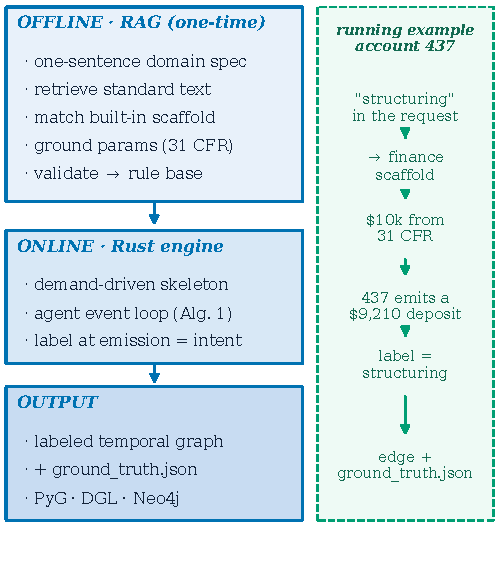
\includegraphics[width=\columnwidth]{fig_architecture.pdf}
\caption{\sys{} end to end, in the order it runs: offline retrieval compiles a typed
rule base (top), the Rust engine simulates a typed agent world into a labeled temporal
graph (middle), and the output loads in common tools (bottom). The lane on the right
follows the running example, account 437's \$9{,}210 structuring deposit, across the
pipeline.}
\label{fig:arch}
\end{figure}

%% =====================================================================
\subsection{From Standards to Rules}
\label{sec:rag}
Step (1) above loaded a rule base; this section is where it comes from.

In \sys{}, a domain is fully determined by its rule base. The rule base states seven
things: what node types exist, what relations connect them, what events occur, what
normal behavior looks like, what legality constraints hold, what anomalous techniques
exist, and a handful of control parameters. The engine consumes only this object, so a
new domain is a new rule base and nothing else.

A rule base holds two kinds of thing, and \sys{} treats them separately:
\emph{structure} and \emph{concrete numbers}. The \emph{structure} is the skeleton:
that the domain has roles like accounts and institutions, that events like transfers
and deposits happen between them, and what an anomaly looks like. We write this part by
hand, once per domain, as a \emph{template}: a fill-in-the-blanks blueprint whose frame
is fixed and whose numbers are left open. The engine's validator checks each template
to be sure it is legal, and six domains are six such templates. The \emph{concrete
numbers} are the thresholds, code sets, and ranges that make a domain realistic: how
much counts as a large amount, which billing-code pairs are mutually exclusive, which
funds count as high-risk. Where a standard legislates such a value, \sys{} reads it out
rather than choosing it: the \$10{,}000 cash-transaction reporting threshold, for
instance, comes straight from U.S.\ regulation 31 CFR 1010.311. Standards legislate
thresholds and ranges but, by design, not an adversary's operational tempo; 31 CFR
defines structuring rate-free, as transactions kept below the threshold ``in any amount
\dots\ on one or more days,'' so that it cannot be gamed by a numeric test. The shape of
a structuring campaign around that grounded threshold, a ring making several
sub-threshold deposits within a short window, is therefore our modelling of the
typology, stated as such, not a value the standard supplies.

The standard supplies
\emph{rules and ranges}, not the value on any individual edge. It tells us that an
amount between \$7{,}000 and \$10{,}000 is suspicious; at generation time, the concrete
amount of a suspicious deposit (say \$9{,}210) is then \emph{sampled at random} from
that range. The standard fixes the rules of the game and the ranges; the engine
generates each edge at random within them.

How does ``reading the standard'' actually work? It is an \emph{offline} pipeline, run
once when the rules are prepared, entirely separate from the fast per-edge generation
that follows. It first gathers the authoritative documents (anti-money-laundering from
the FATF recommendations and the U.S.\ Bank Secrecy Act, cybersecurity from MITRE
ATT\&CK, medical billing from the CMS coding edits, and so on), stored by source. Given
a one-sentence description of the domain the user wants, a
retriever~\cite{robertson2009bm25,johnson2021faiss,lewis2020rag} pulls the relevant
passages; \sys{} picks the matching domain template, then fills the template's open
numbers from those passages, tagging each number with the source span it came from so
it stays traceable. This step is done mainly by rule-based extraction; only when the
extraction misses a number does a small open language model~\cite{qwen2024report} fill
it in. The language model is thus an optional helper, not the author: the numbers come
from the standard text, and whether the resulting rule base is legal is decided by the
engine itself. Because of this, the size of the language model barely affects the
result (\S\ref{sec:exp} verifies this directly). In Listing~\ref{lst:rule}, for example,
the \$10{,}000 reporting threshold is read from 31 CFR 1010.311 rather than chosen by the
model; the surrounding campaign shape is our modelling of the typology (\S\ref{sec:rag}).

Because rule synthesis is a one-time, offline step that never touches the per-edge
path, generation can reach millions of edges per second. To change domains, one only
changes the corpus: the same program picks the matching template and re-fills its
numbers from the new documents. The curated corpus is itself a reusable artifact.

\begin{lstlisting}[float=t,caption={The compiled \texttt{cash\_deposit} rule (finance,
abridged). The hierarchical \texttt{channel} taxonomy and the graded
\texttt{source\_of\_funds\_grade} give the edge its multi-level attributes; the
\$10k threshold is grounded in 31 CFR while the campaign shape around it is a modelling
choice.},label={lst:rule}]
event cash_deposit:              # account -> institution
  channel: !taxonomy             # hierarchical, coarse -> fine
    cash/domestic/small_bills     0.34
    cash/domestic/large_bills     0.15
    wire/inbound_cross_border     0.10   # (7 paths total)
  source_of_funds_grade: !ordinal        # graded AML risk tier
    payroll_documented ... high_risk_corridor
  amount: !log_normal(mu=5.8, sigma=1.2)

constraint ctr_structuring_window:       # 31 CFR 1010.311
  >= 4 cash_deposit in [$7k, $10k] within 7 days
\end{lstlisting}

%% =====================================================================
\subsection{The Simulation Engine}
\label{sec:engine}
The engine's core is written in Rust (memory safety matters for a tool that others
download, that parses untrusted rule bases, and that runs massively parallel); a thin
Python layer only handles configuration, the offline retrieval, and plotting.

\subsubsection{Population, state, and the event loop}
\label{sec:loop}
Generation is a discrete-event simulation~\cite{banks2010des}: its cost grows with
the number of \emph{events}, not with (time steps)$\times$(agents), which is what
lets a year of activity for millions of agents run in seconds. After the population
and skeleton are built (\S\ref{sec:overview}), every agent is given a first action
time drawn from its behavior's rate and diurnal shape, and these are placed in a
per-block event queue. The main loop (Alg.~\ref{alg:loop}) repeatedly takes the
earliest pending action, asks the responsible process what to do, emits the resulting
edge, applies its effect on node state, and reschedules the agent's next action.
Although each step is pure numerics, the agents do not emit numbers in isolation but
depend on one another through \emph{shared node state}. A
transfer debits the source account and credits the destination, so later actions and
legality checks see the modified state, and interdependent outcomes like an
insufficient balance or a frozen account arise naturally.

Concretely, the anomalous account 437 wakes one Monday morning; the loop picks a
cash-deposit event for it with branch 812 as the counterparty, samples a \$9{,}210
amount, emits an edge labeled \textsf{structuring} (because a structuring process fired
it), records the money against the relevant balances, and reschedules 437's next
action. Timestamps are organized in causal blocks (e.g.\ days); within a block, agents
are independent and run in parallel, and a splittable counter-based
generator~\cite{salmon2011random123} makes the output \emph{bit-identical across any
thread count}, the guarantee that lets a distributed run reassemble exactly
(\S\ref{sec:exp}).

Two mechanisms carry the realism. \emph{Counterparty
selection} (line 5) chooses \emph{whom} an agent acts on, and it is the per-event hot
path, so it must be $O(1)$: an agent either reuses a recent partner (building the
repeated edges that give real burstiness and reciprocity), draws a fresh neighbor from
its skeleton relation, or samples a popularity-weighted hub from an alias
table~\cite{walker1977alias,vose1991alias} (so hubs accrue degree without any neighbor
scan). \emph{State effects} (line 8) keep the world coherent: a transfer subtracts its
amount from the source balance and adds it to the destination, a deposit raises a
balance, a login marks a host compromised, so later actions and legality checks see a
consistent history and cascading consequences (a frozen account, a compromised subnet)
arise naturally rather than being scripted.

\begin{algorithm}[t]
\caption{\sys{} generation (one causal block, run per thread)}
\label{alg:loop}
\small
\begin{algorithmic}[1]
\STATE \textbf{input:} rule base $\mathcal{R}$; population $V$; skeleton $\mathcal{S}$; queue $Q$
\WHILE{$Q$ not empty}
  \STATE $(a,t) \gets Q.\text{pop\_min}()$ \hfill// earliest pending action
  \STATE $p \gets \textsc{ActiveProcess}(a)$ \hfill// normal behavior, or an adversary stage
  \STATE $\varepsilon \gets p.\text{event}$;\; $v \gets p.\textsc{Counterparty}(a,\mathcal{S})$ \hfill// $O(1)$ alias
  \STATE $\mathbf{a} \gets p.\textsc{SampleAttrs}(\varepsilon)$;\; $\ell \gets \iota(p)$ \hfill// label $=$ intent
  \STATE \textbf{emit} edge $(a, v, t, \mathbf{a}, \ell)$
  \STATE \textsc{ApplyEffects}$(\varepsilon, a, v)$ \hfill// e.g.\ balance $-$/$+$
  \STATE $\Delta t \sim p.\text{timing}$;\; $Q.\text{push}(a,\, t{+}\Delta t)$
\ENDWHILE
\end{algorithmic}
\end{algorithm}

\subsubsection{Graded and hierarchical attributes}
\label{sec:attrs}
Real records are not flat: a deposit is not merely an amount but a tendered
\emph{kind} of money. \sys{} therefore lets any attribute be \emph{hierarchical} or
\emph{graded}, alongside numeric and categorical fields. Account 437's deposit in
Table~\ref{tab:trace} makes this concrete: its \texttt{channel} is
\texttt{cash/domestic/small\_bills}, a \emph{hierarchical} path that runs coarse to fine
(cash, then domestic, then small bills) and rolls up to any level by prefix; and its
source-of-funds grade is an ordinal tier from ``payroll-documented'' up to ``high-risk
corridor,'' a \emph{graded} attribute. It is these, together with the amount, that form
the FATF/FinCEN structuring signature: the label lives in the \emph{conjunction} of the
channel path, the risk grade, and the amount band, not in the amount alone. This
matters because modern anomaly detectors do not key on coarse aggregates but on the
interaction of fine-grained, multi-level features, and aggregation destroys exactly that
signal. Graded attributes also give the difficulty axis a finer surface: as camouflage
rises, an adversary's deposits regress toward the benign channel and grade distribution,
so a detector must combine levels rather than threshold one number.

\subsubsection{The interaction skeleton}
\label{sec:substrate}
The skeleton fixes who \emph{can} interact before anyone acts: which accounts might
transfer to each other, which hosts a process might reach. \sys{} lays it down with a
standard topology model chosen per domain, a preferential-attachment or
affiliation backbone for hub-and-spoke settings like finance and crypto, small-world for
road and forum structure, so that an agent's $O(1)$ counterparty draw is biased toward
plausible partners through an alias table without any neighbour scan. These same models
(BA, R-MAT, SBM, spatial, affiliation) are also the baselines \sys{} is measured against
(\S\ref{sec:compare}). The point of \sys{} is not the backbone but what runs on it: the
observable transaction graph grows as agents act, and it is that activity, not the
topology alone, that supplies the time, recurrence, and labels a formula misses, which is
why \sys{} reaches fidelity $0.79$ against a real interaction network where the same
backbone with random timestamps reaches only $0.64$ (\S\ref{sec:compare}).

\subsubsection{Scaling to enormous graphs}
\label{sec:scaling}
The cost of generation is $O(|E|)$: the event loop performs one iteration per edge,
and each iteration is $O(1)$, an alias draw for the counterparty, a constant-size
attribute sample, and a constant-size state update. The only super-linear step is
an optional final sort of edges into global time order, $O(|E|\log|E|)$, which is
also the throughput bottleneck in practice (\S\ref{sec:exp}). Within a causal time
block, agents do not depend on one another, so the loop is data-parallel across
cores.

Across \emph{machines}, \sys{} parallelizes naturally: each machine independently does
its own share, and the machines need \emph{no communication during generation}
(Alg.~\ref{alg:dist}). Each of $N$ machines runs the same program with the same seed
but simulates only the nodes whose id is congruent to its rank modulo $N$, emitting
only the edges those nodes source; the result is a set of disjoint shards whose union
is the whole graph. No communication is needed because every random draw comes from a
counter-based generator~\cite{salmon2011random123} keyed by the node id and event
index, so a node's entire event sequence is the same no matter which machine computes
it or how its threads interleave, and the shards align by construction. Would the
machines ever need to reconcile? Not during generation; reconciliation is something we
do only in \emph{post-hoc verification}, merging the shards and comparing bit-for-bit
against a single-machine run (\S\ref{sec:exp} does this for a four-shard run, whose
union is md5-identical to the single-machine graph). Per-machine memory and work
therefore fall as $O(|V|/N)$ and $O(|E|/N)$: the more machines, the lighter each one's
load, which is what makes billion- and trillion-edge targets reachable.

\begin{algorithm}[t]
\caption{Distributed generation on $N$ machines (no coordination)}
\label{alg:dist}
\small
\begin{algorithmic}[1]
\REQUIRE identical seed and rule base $\mathcal{R}$ on every machine
\STATE \textbf{machine} $k$: $\;V_k \gets \{\,v : \mathrm{id}(v)\bmod N = k\,\}$
\STATE instantiate $V_k$; each draw uses an RNG substream keyed by $(\mathrm{id}(v),\text{ event\#})$
\STATE run Alg.~\ref{alg:loop}, emitting only edges whose source is in $V_k$
\STATE write shard $k$ \hfill// shards are disjoint by source node
\ENSURE $\textstyle\bigcup_k \text{shard}_k$ equals the single-machine graph, bit-for-bit
\end{algorithmic}
\end{algorithm}

\subsubsection{Introspection and deployment}
Edges stream to sharded columnar files. A single pass computes degree, clustering,
temporal-density and attribute summaries with streaming
sketches~\cite{flajolet2007hyperloglog,cormode2005countmin} and exposes a
\texttt{/metrics} endpoint, so a billion-edge run is measurable \emph{without a second
pass}. Because the simulator knows every label, the anomaly composition is exact and
free. \texttt{agora doctor} probes the host (cores, RAM, GPU, disk) and
\texttt{--dry-run} estimates time, memory and disk before committing, so the tool runs
across different platforms. Distributed runs shard by node id (\S\ref{sec:exp}).

\paragraph{Reproducibility and use.}
Every run writes a \texttt{meta} file recording the exact configuration, the seed, the
engine version, and the host, so a result is reproducible to the edge: the seeded
splittable generator guarantees the \emph{same} graph from the same \texttt{meta}, on
any thread count or machine. Data is emitted in Parquet, CSV, or GraphML, loadable
directly by PyG, DGL, Neo4j and igraph with no preprocessing, alongside the
\texttt{ground\_truth.json} campaign records and node-level labels. The tool installs
as a Python wheel (\texttt{pip install agora}), a prebuilt binary, or from source. From
a one-sentence description of a domain, a user obtains a loadable, labeled benchmark,
which shifts a practitioner's effort from \emph{acquiring} labeled temporal-graph data,
which barely exists, to \emph{specifying} it.

%% =====================================================================
\subsection{Anomalies: Emergence, Labels, and Difficulty}
\label{sec:anom}
\paragraph{What an anomaly is here.}
``Anomaly'' conflates three ideas that a \emph{generator} must keep
apart~\cite{hawkins1980identification,chandola2009anomaly}: an observation from a
\emph{different mechanism}; a \emph{rule violation}; and a \emph{surprise} to some
model. Only the last is affected by whether we ``know'' the label. \sys{} anchors
truth to the first: an anomaly is an edge produced by a different generative
process (a fraudster, a failing sensor), and its label records \emph{which}
process, never a post-hoc rule check. A legality constraint (e.g.\ a balance must
stay non-negative) is available as a detector's-eye feature, but it is not the
ground truth.

\paragraph{How an anomaly emerges.}
An adversarial process is an ordinary agent with a goal and a staged plan. A
structuring campaign, for instance, recruits a small ring of accounts and runs two
stages: a \emph{smurf} stage in which each member emits many sub-\$10{,}000 cash
deposits, and an \emph{aggregate} stage in which the ring funnels the money to one
collector account (a fan-in). These stages emit real edges into the same event
loop as everyone else (Alg.~\ref{alg:loop}); the campaign is anomalous not because
we tagged its edges but because a laundering agent, not a shopper, produced them.
Every such edge carries an identifier joining it to the campaign record in
\texttt{ground\_truth.json}, so labels are available at the edge, node, and
subgraph level, the multi-level ground truth detectors actually need. When account
437's \$9{,}210 deposit is emitted the simulator writes \textsf{structuring} not because
the amount tripped a threshold but because the edge came from the ring's smurf
stage, the same fourteen deposits and the fan-in onto collector 951 would be
indistinguishable from three ordinary customers banking cash had a normal process
produced them.

\paragraph{Controlling rate and difficulty.}
An edge $e_i$ is produced by exactly one process $p_i$, and
\begin{equation}
\ell_i=\iota(p_i),\qquad r=\Pr[\ell_i\neq\textsf{normal}]=g(\pi),\label{eq:rate}
\end{equation}
so the anomaly \emph{rate} $r$ is a function of the anomalous-agent prevalence
$\pi$, set by how many agents are adversarial and how active they are, never by
fixing a count of ``bad'' edges after generation. $g$ is monotone by
construction, more adversarial agents, or more active ones, can only add
anomalous edges, and empirically near-linear (\S\ref{sec:exp}). To hit a target
\emph{edge}-level rate $r^\star$ rather than a population $\pi$, a short calibration
pass measures $g$ on a small pilot run and inverts it, $\pi=g^{-1}(r^\star)$, then
rescales normal-agent activity so the total edge budget is met; because $g$ is
monotone this needs no search. Nothing here fixes \emph{which} edges are
anomalous, only how many agents misbehave, so labels remain a byproduct
of who acted. \emph{Difficulty} is a separate knob $\delta\in[0,1]$ that makes
anomalies harder to catch, and it does so along \emph{two} axes at once. On
\emph{attributes}, with probability $\delta$ the adversary's override is dropped and the
value is drawn from the normal population instead,
\begin{equation}
\theta_p(\delta)=(1-\delta)\,\theta_p+\delta\,\theta_{\textsf{normal}},\label{eq:camou}
\end{equation}
so the deposit's amount and channel come to look like ordinary business. On
\emph{structure}, with the same probability the edge is rerouted to a benign
counterparty, diluting the ring or fan-in motif so that a structure-aware detector
degrades too. This is \emph{camouflage}: at $\delta{=}0$ a structuring deposit is a
blatant round sub-threshold amount wired cleanly onto the collector; at $\delta{=}1$ its
amount looks like ordinary business and its edge scatters like normal traffic. The label
never changes, only how separable the edge is from normal, which is exactly the
property that makes a benchmark easy or hard, and which we measure in \S\ref{sec:exp}.
Two further knobs govern where anomalies land: one concentrates them in chosen
communities or time windows, and one lets a finished campaign spawn a follow-up with
probability $\mathit{cascade\_p}$. Cascades model a real effect: these events
self-excite and spread in time (a jammed road segment jams its neighbors, a compromised
host pivots laterally), so we calibrate the self-excitation shape against real
interaction data and set its strength per domain.

%% =====================================================================
\subsection{The Six Domains}
\label{sec:domains}

\paragraph{The same machinery, grounded per domain.}
The structuring campaign is not special-cased; it is one instance of a general
pattern in which a domain's adversarial \emph{processes are its standard's own named
typologies}. The finance ring enacts FATF's placement-and-layering typology; the
cyber adversary walks MITRE ATT\&CK tactics (initial access, lateral movement,
exfiltration) as staged events over hosts and accounts; healthcare upcoding and
kickback rings follow the CMS NCCI edit pairs and the anti-kickback pattern; crypto
wash trading, mixing, and rug pulls follow the exchange-surveillance typologies; and
e-commerce review fraud follows the coordinated-reviewer pattern. In every case the
adversary is an ordinary agent with a goal and a staged plan emitting real edges into
the shared event loop (Alg.~\ref{alg:loop}); its label is the intent of the process,
and its rate and difficulty obey Eqs.~\eqref{eq:rate} and~\eqref{eq:camou} unchanged. Switching domains therefore
does not switch mechanisms, only which typology the offline corpus supplies.

\paragraph{Six built-in domains.}
Six rule bases ship with \sys{}, each grounded in the standards of \S\ref{sec:rag}.
Five are adversarial; transportation is deliberately \emph{non}-adversarial, its
anomalies are congestion cascades and sensor faults, modeled as \emph{failure}
processes rather than intents, which stresses that the same seven-part schema
expresses natural anomalies too, not only fraud. Four domains are validated against a
domain-matched real temporal graph and two (transport, healthcare) against a structural
proxy, for lack of a public match (\S\ref{sec:exp}). Table~\ref{tab:domains} lays the
six side by side with their anomaly source, representative playbooks (the intent
labels), and grounding standards.

\begin{table*}[t]
\caption{The six built-in domains: one engine and one seven-part schema, each domain
only a rule base grounded in named, public standards. ``Source'' is whether a domain's
anomalies are adversarial intents or natural failures; a playbook is a staged agent
policy, not an injected motif. Fidelity against real temporal graphs is in
Table~\ref{tab:fidelity}.}
\label{tab:domains}
\small\centering
\resizebox{\textwidth}{!}{%
\begin{tabular}{@{}llll@{}}
\toprule
domain & anomaly source & representative playbooks (intent labels) & grounding standards \\
\midrule
finance/AML & adversarial & structuring, layering, fan-in/out, round-trip, mule ring & FATF, FinCEN 31 CFR \\
crypto & adversarial & wash trading, phishing drain, mixing, rug pull, Ponzi & Etherscan, ERC-20 \\
cybersecurity & adversarial & port scan, brute force, lateral movement, C2 beacon, exfiltration & MITRE ATT\&CK \\
transportation & \emph{natural} & congestion cascade, incident, sensor fault & HCM \\
e-commerce & adversarial & fake reviews, collusion ring, sockpuppets, return fraud & FTC 16 CFR 465 \\
healthcare & adversarial & upcoding, phantom billing, kickback ring, doctor-shopping & CMS NCCI \\
\bottomrule
\end{tabular}}
\end{table*}

\paragraph{Reading the table.}
Three things stand out. First, one engine and one seven-part schema span six domains as
different as finance and healthcare, changing only the rule base and not a line of
engine code. Second, each domain's playbooks are not invented ad hoc: each maps to a
public, checkable named standard (FATF, MITRE ATT\&CK, CMS NCCI, and so on), so ``what
counts as an anomaly'' is grounded rather than a matter of taste. Third, the source
column shows the same machinery expressing both intentful adversaries (five domains) and
intentless natural faults (transportation), so the definition ``an anomaly is an edge
from a different process'' reaches beyond fraud.

%% =====================================================================
\section{Evaluation}
\label{sec:evaluation}

\subsection{How We Evaluate}
\label{sec:eval}
Judging the quality of a generated benchmark takes more than reading a degree plot.
LDBC's influential methodology checks structural realism and query ``choke points''
(the hard queries that stress a database)~\cite{boncz2013tpch,erling2015ldbc}; it has
no notion of temporal-graph realism, is unconcerned with downstream utility, and,
carrying no labels, has nothing to say about how hard an anomaly is to catch. \sys{}
evaluates a generated dataset along five concrete axes, and states its aggregate up
front.

\paragraph{Fidelity, defined.}
We compute the same battery of statistics on a real graph $R$ and a synthetic graph
$S$ and report a transparent aggregate
\begin{equation}
\mathrm{fid}(S,R)=1-\frac{1}{|\mathcal{M}|}\sum_{m\in\mathcal{M}} d_m(S,R)\in[0,1],\label{eq:fid}
\end{equation}
where every per-metric distance $d_m\in[0,1]$: for \emph{distributional} metrics
(in/out/total degree, inter-event times) $d_m$ is the two-sample Kolmogorov--Smirnov
statistic~\cite{massey1951ks}, a standard measure of how far two distributions lie
apart; for \emph{scalar} metrics (power-law exponent, burstiness $B$, memory,
clustering, reciprocity, repeat rate) $d_m$ is a bounded normalized difference. We
report the components, not only the sum, because a single number hides a great deal, as
\S\ref{sec:compare} shows. What each metric captures is listed in
Table~\ref{tab:metrics}.

\begin{table}[t]
\caption{What each fidelity metric captures. Distributional metrics are compared by a
two-sample KS statistic, scalar metrics by a bounded normalized difference.}
\label{tab:metrics}
\footnotesize\centering
\setlength{\tabcolsep}{3pt}
\begin{tabular}{@{}>{\raggedright\arraybackslash}p{0.28\columnwidth} >{\raggedright\arraybackslash}p{0.60\columnwidth} l@{}}
\toprule
metric & what it captures & type \\
\midrule
degree (in/out/total) & how many edges a node has, and how heavy the hub tail is & dist. \\
inter-event time & the gap between a node's consecutive actions & dist. \\
power-law exp.\ \cite{clauset2009powerlaw} & how heavy the degree tail is (hub extremity) & scalar \\
burstiness $B$ \cite{goh2008burstiness,kim2016burstiness} & whether events cluster in bursts or spread evenly & scalar \\
memory \cite{goh2008burstiness} & whether a long inter-event gap tends to be followed by another long gap & scalar \\
clustering \cite{watts1998smallworld} & how often two neighbors of a node are themselves linked & scalar \\
reciprocity & fraction of $A\!\to\!B$ edges that have a reverse $B\!\to\!A$ & scalar \\
repeat rate & fraction of node pairs linked more than once & scalar \\
\bottomrule
\end{tabular}
\end{table}

\paragraph{Controlling for confounds.}
Fidelity evaluation should first neutralize artifacts of how a \emph{real} benchmark
was prepared, or it measures preprocessing rather than realism. Three recur. First,
some curated benchmarks \emph{k-core filter}~\cite{seidman1983kcore} away low-degree
nodes (TGB keeps $k\!\ge\!5$); comparing an unfiltered synthetic graph against a
filtered real one inflates the gap between the two degree distributions, since the
low-degree nodes are still present in the synthetic graph but were deleted from the real
one, so our harness applies the same filter to both. Second, a single network capture
(e.g.\ one day of CICIDS) has its own idiosyncratic, fixed topology, a handful of server
hubs; a domain-agnostic generator produces a different topology and the two will not
match, so we report that difference rather than count it as a defect. Third, a
multi-relation synthetic output is projected to the matching relation before comparison
to a single-relation real dataset, or the repeat-edge rate does not line up: in a
multi-relation graph one pair of nodes may be connected repeatedly under several
different relations, and without the projection those edges from other relations are
counted too, inflating the repeat rate. More than once we found that an ``obvious''
generator fix was addressing a problem that was not there, one that lived in the
preprocessing and not the generator. We therefore build the measurement instrument
first and control these confounds.

\paragraph{The five axes.}
\emph{Structure} (L1): MMD~\cite{gretton2012mmd} over degree, clustering, and orbit
(a node's role in small subgraphs~\cite{hocevar2014orca}) distributions, with the
positive-definite-kernel and perturbation-monotonicity safeguards
of~\cite{obray2022evalmetrics,you2018graphrnn} that keep the distance itself reliable.
\emph{Statistics} (L2): energy and Wasserstein~\cite{villani2009ot} distances. The
energy distance is a statistical distance between two distributions computed from
pairwise sample distances, zero exactly when the two agree, and equal to MMD under a
particular kernel~\cite{sejdinovic2013energy}; we also fit power laws by the principled
maximum-likelihood method~\cite{clauset2009powerlaw} rather than a straight line on a
log-log plot. \emph{Temporal dynamics} (L3): the temporal-motif
fingerprint~\cite{paranjape2017motifs} and burstiness with finite-size
correction~\cite{goh2008burstiness,kim2016burstiness}. LDBC does not cover this axis,
and a static generator cannot match it even with timestamps sprinkled on.
\emph{Downstream utility} (L4): a test of whether a
\emph{temporal GNN} trained on the data learns as it would on real data. We train a
TGN~\cite{rossi2020tgn} on future link prediction and report test average precision
(\S\ref{sec:exp}); we also run a classifier two-sample test~\cite{lopezpaz2017c2st} on
how distinguishable synthetic edges are from real. \emph{Anomaly difficulty} (L5):
because \sys{} emits exact labels, we train a detector on a generated graph and
\emph{measure} how its accuracy falls as the difficulty knob rises, the control
of~\cite{emmott2013anomaly} made concrete, which addresses the standing complaint that
fixed anomaly benchmarks carry trivial or mislabeled
positives~\cite{wu2021flawed,han2022adbench}. Privacy and disclosure metrics
(distance-to-closest-record, membership inference~\cite{vanbreugel2023domias}), relevant
because we release data, are provided by the harness and left to future evaluation.

%% =====================================================================
\subsection{Comparison with Other Generators}
\label{sec:compare}
We compare \sys{} directly against the classical generators it replaces, matched to a
real temporal graph's node and edge count. None of them emit timestamps, so we give them
the treatment a practitioner would, uniform-random timestamps over the real span, which
is what reveals how far bare topology is from a real temporal graph. All are scored with
the identical battery of \S\ref{sec:eval} against the same real target.

\paragraph{Capabilities first.}
Table~\ref{tab:caps} summarizes what each generator can produce. Only real data
and \sys{} carry all six of temporal edges, rich attributes, anomaly labels, a
controllable difficulty knob, zero-code multi-domain coverage, and $10^8$-edge scale.
Many of the real temporal graphs we compare against carry no rich attributes or labels
themselves, so on the ``rich attributes'' row \sys{} supplies something the real
reference graphs lack; this is also why the fidelity we report covers structure and time
only, with attribute-distribution fidelity having nothing to compare against and left
unmeasured. Every classical generator produces topology only; LDBC adds semantics but no
labels; AMLSim injects labels but in one small hand-built domain; learned temporal
generators neither scale nor control difficulty. The gap is in capability, not in a
decimal place of fidelity.

\paragraph{Versus LDBC: generality by construction.}
The generators above fall into a few families by capability: formula-based generators
that produce topology only (BA, R-MAT), simulation-based generators with good semantics
but hand re-targeting (AMLSim), learned generators that chase quality but do not scale
(CTGAN, TIGGER), and curated benchmarks that are real but not generative (TGB, LDBC). We
single out the one closest to \sys{} in ambition, LDBC's Social Network Benchmark
Datagen~\cite{erling2015ldbc,pham2012s3g2}, the de-facto standard for graph-database
benchmarking. It is a product of extensive \emph{hand} engineering: the benchmark council and
domain experts designed one carefully correlated social-network schema (persons, forums,
posts, \textsf{knows} edges) with skewed, structure-correlated distributions and
choke-point-driven queries. That craftsmanship is also its boundary: it covers one
business domain. Re-targeting LDBC to finance, healthcare, or cybersecurity means
re-designing the schema, the correlations, and the generator by hand, because its domain
knowledge lives in \emph{code written by people}. \sys{} inverts this. The domain
knowledge lives in \emph{retrieved published standards} (\S\ref{sec:rag}), so a new
domain is a new \emph{corpus}, not new code; the single binary in this paper produces
all six. \sys{} trades a little of LDBC's hand-tuned per-domain polish for \emph{zero-code
domain migration}, plus the anomaly labels, attributes, and difficulty control LDBC never
targeted. The two are complementary: LDBC for deep single-domain query benchmarking,
\sys{} for labeled, multi-domain, temporal-graph learning.

\begin{table}[t]
\caption{What each generator can produce. Only real data and \sys{} are complete
(inj.\ $=$ injected templates; -- $=$ N/A: TGB curates real data).}
\label{tab:caps}
\scriptsize\centering
\setlength{\tabcolsep}{3.2pt}
\resizebox{\columnwidth}{!}{%
\begin{tabular}{@{}lccccccc@{}}
\toprule
 & BA/R-MAT & LDBC & AMLSim & CTGAN & TGB & TIGGER & \sys \\
\midrule
power-law/comm. & \cmark & \cmark & \pmark & \xmark & -- & \pmark & \cmark \\
temporal edges & \xmark & \cmark & \cmark & \xmark & \cmark & \cmark & \cmark \\
rich attributes & \xmark & \pmark & \cmark & \cmark & -- & \xmark & \cmark \\
anomaly labels & \xmark & \xmark & inj. & \xmark & \pmark & \xmark & \cmark \\
ctrl.\ difficulty & \xmark & \xmark & \xmark & \xmark & \xmark & \xmark & \cmark \\
multi-domain & \xmark & \xmark & \xmark & \pmark & \cmark & \xmark & \cmark \\
scale $\ge 10^8$ & \cmark & \cmark & \xmark & \xmark & -- & \xmark & \cmark \\
\bottomrule
\end{tabular}}
\end{table}

\paragraph{The full contest: every generator, every domain (Fig.~\ref{fig:matrix}).}
We pit \sys{} against \emph{nine} other generators on all six domains, each matched to
a real temporal graph and scored by fidelity (Fig.~\ref{fig:matrix}). The field splits
in two. \emph{Prior} generators (Barab\'asi--Albert, R-MAT,
Kronecker~\cite{leskovec2010kronecker}, Watts--Strogatz, Erd\H{o}s--R\'enyi, and
\sys) synthesize a graph \emph{without ever seeing the target}. \emph{Fit-to-real}
generators (the configuration model, Chung--Lu, a degree-corrected
SBM~\cite{karrer2011dcsbm}, and a random dot-product graph, RDPG~\cite{athreya2018rdpg})
are instead \emph{handed} the real graph's own degree sequence or adjacency
spectrum and rebuild from it, which a benchmark generator cannot do (it would need the
very graph it is meant to synthesize). Two patterns hold across the matrix. First, the \emph{fit-to-real} generators are
generally strongest on raw structural fidelity, unsurprisingly, as they are handed
the target's degree sequence or spectrum; the configuration model has the highest mean
($\approx\!0.85$). But this is fidelity \emph{to a degree sequence}, which is necessary
and nowhere near sufficient: it wins on degree yet misses clustering, reciprocity, and
time, and, like every generator here except \sys{}, carries no attributes and no
labels (Table~\ref{tab:caps}). Second, among the
\emph{prior} generators that build a graph \emph{blind}, \sys{} is the strongest on
four of six domains (finance, crypto, cyber, healthcare) and close on the other two,
where R-MAT edges it (transport $0.77$ vs.\ $0.70$; e-commerce $0.863$ vs.\ $0.861$).
On crypto, \sys{} beats every generator, including the fit-to-real ones ($0.84$ vs.\
their best $0.83$), without ever seeing the graph. Across all six domains its structural
fidelity ($0.70$--$0.86$) sits in the same band as methods that were shown the answer.
To our knowledge, \sys{} is the only generator that reaches this band \emph{without the
real graph in hand} while carrying the time, attributes, and labels a benchmark needs.

\paragraph{Why, zoomed in on one graph (Table~\ref{tab:baselines}).}
Decomposing one matched pair (CollegeMsg, a real messaging network with 1{,}899 nodes
and 59{,}835 edges) shows where the gap to a formula lies: \sys{} recovers reciprocity
($0.12$ vs.\ a real $0.64$; BA gives $0.000$), burstiness ($0.42$ vs.\ $0.68$), and
clustering far better than BA/ER/WS, reaching fidelity $0.79$ against their
$0.56$--$0.71$ (Table~\ref{tab:baselines}). The configuration model's $0.82$ is higher
only because it is handed the degree sequence, and it still gets clustering
$2.8\times$ too high and carries no semantics. This is why we report components, not a
scalar, and why fidelity spans seven real graphs in four domains (Table~\ref{tab:fidelity}).

\begin{table}[t]
\caption{\sys{} vs.\ classical generators, matched to CollegeMsg and scored against
it. Only real data and \sys{} carry attributes/labels.}
\label{tab:baselines}
\small\centering
\resizebox{\columnwidth}{!}{%
\begin{tabular}{@{}lrrrrc@{}}
\toprule
generator & clust. & recip. & burst.\ $B$ & fidelity & att./lab. \\
\midrule
real (reference) & 0.138 & 0.636 & 0.676 & 1.000 & \cmark \\
\textbf{\sys{} (ours)} & 0.086 & 0.124 & 0.416 & \textbf{0.793} & \cmark \\
Erd\H{o}s--R\'enyi & 0.033 & 0.015 & 0.000 & 0.558 & \xmark \\
Barab\'asi--Albert & 0.084 & 0.000 & 0.300 & 0.642 & \xmark \\
R-MAT & 0.184 & 0.101 & 0.311 & 0.705 & \xmark \\
config.\ model$^\dagger$ & 0.388 & 0.190 & 0.000 & 0.816 & \xmark \\
Watts--Strogatz & 0.543 & 0.000 & 0.691 & 0.557 & \xmark \\
\bottomrule
\end{tabular}}\\[2pt]
{\footnotesize $^\dagger$given the real degree sequence; matches degree by design.}
\end{table}

\begin{figure*}[t]
\centering
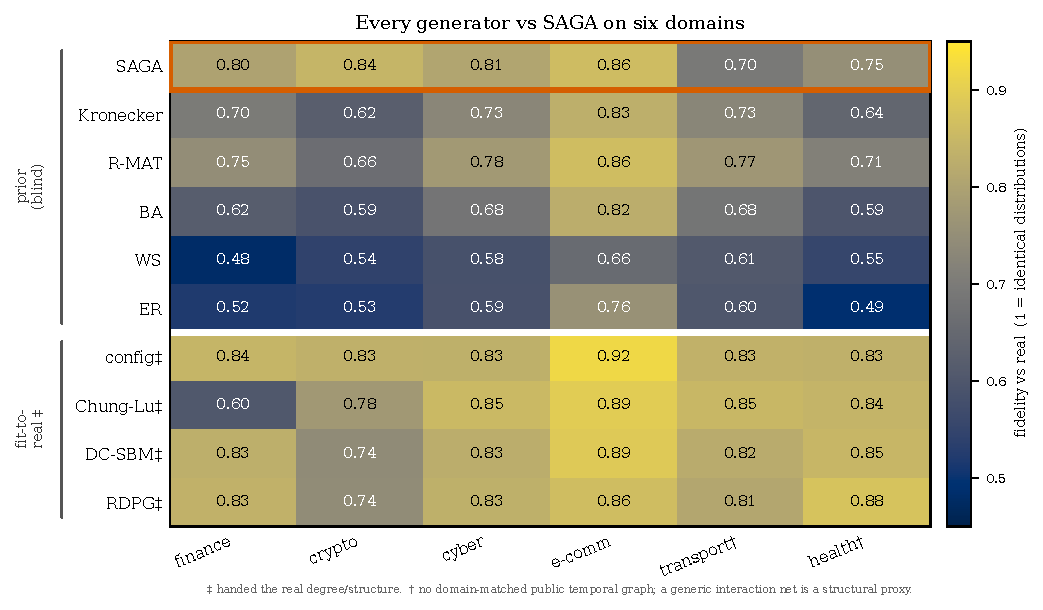
\includegraphics[width=\textwidth]{fig_matrix.pdf}
\caption{\textbf{Fidelity on all six domains.} Ten generators (rows) vs.\ a matched real
temporal graph per domain (columns); darker\,$=$\,closer to real. \emph{Fit-to-real}
($\ddagger$) are handed the target's degree sequence or spectrum; \sys{} is boxed.
$\dagger$structural proxy (no domain-matched public graph exists).}
\label{fig:matrix}
\end{figure*}

\paragraph{And the learned generators (Table~\ref{tab:learned})?}
The deep and tabular generative models cannot be run at the scales
above: TIGGER~\cite{gupta2022tigger} is transductive (a parameter row per node,
$\sim\!10^3$ nodes on CPU), and CTGAN/TVAE~\cite{xu2019ctgan} are topology-blind
(they fit the degree \emph{marginal}, not who-connects-to-whom). We therefore compare
them on a controlled $2{,}500$-node slice of each domain (Table~\ref{tab:learned}).
There they are competitive on fidelity (CTGAN and the configuration model even exceed
\sys), but a single fidelity number hides three catches. First, every one of them is
\emph{trained on the target graph}: like the configuration model they are
fit-to-real, and a benchmark generator should not need the very graph it is meant to
synthesize. Second, they \emph{do not scale}: the models that took a minute on
$25$k edges cannot reach the $10^9$ edges of Table~\ref{tab:scale}. Third, they carry
\emph{no} anomaly labels, attributes, or difficulty control, and must be retrained for
every new dataset. To our knowledge, \sys{} is the only generator that reaches
competitive fidelity \emph{without the target graph}, scales to a billion edges, and
emits ground-truth labels; it defines a domain once rather than fitting a dataset.

\begin{table}[t]
\caption{\textbf{Learned generators on a controlled $2{,}500$-node slice} (fidelity;
they cannot run at real scale). They are competitive at toy scale, but all are
\emph{fit-to-real} ($\ddagger$: trained on the target graph), none scale to $10^9$
edges, and none carry labels or attributes.}
\label{tab:learned}
\centering
\resizebox{\columnwidth}{!}{%
\begin{tabular}{@{}lccccccl@{}}
\toprule
method & finance & crypto & cyber & e-comm & transp. & health & max.\ scale \\
\midrule
\textbf{\sys{}}    & .80 & .80 & .84 & .86 & .69 & .78 & \textbf{$10^9$ edges} \\
TIGGER$\ddagger$   & .85 & .80 & .87 & .86 & .86 & .85 & $\sim\!10^3$ nodes \\
CTGAN$\ddagger$    & .86 & .84 & .89 & .88 & .87 & .87 & topology-blind \\
TVAE$\ddagger$     & .84 & .75 & .82 & .88 & .88 & .88 & topology-blind \\
config$\ddagger$   & .84 & .88 & .88 & .93 & .88 & .86 & degree-fed \\
BA                 & .62 & .58 & .74 & .93 & .68 & .64 & any \\
\bottomrule
\end{tabular}}
\\[2pt]
{\footnotesize $\ddagger$ trained on / fed the target real graph. \sys{} is the only
row that needs no access to the real graph, scales to $10^9$ edges, and carries
labels+attributes.}
\end{table}

%% =====================================================================
\section{Experiments}
\label{sec:exp}
All runs are on one 32-thread host (Intel i9-13900K, 24 cores / 32 threads, 62\,GB
RAM); \sys{} is seed-fixed
and bit-reproducible (\S\ref{sec:repro}). The experiments establish five things in
turn. Generation \emph{scales} linearly in edges (Table~\ref{tab:scale}).
The output \emph{matches real data} on the metrics that matter,
reported per metric rather than as one opaque score (Table~\ref{tab:fidelity}). The six
domains are structurally \emph{distinct}, not one graph relabeled
(Table~\ref{tab:multidomain}). The anomaly rate is \emph{controllable}
(\S\ref{sec:exp}), and the difficulty knob is \emph{effective} against a real
detector (Table~\ref{tab:diff}). And the result is \emph{useful downstream}: a temporal
GNN, and a non-learning memorization baseline, learn from it as they would from real
data (Table~\ref{tab:downstream}). Where a domain-matched real reference exists we
compare against it directly, and the results trace to seeded commands in the released
harness.

\paragraph{Speed and scale (Table~\ref{tab:scale}).}
Generation is linear in edges all the way to a \emph{billion}: $10^7$ edges in
$2$\,s, $10^8$ in $17$\,s, and $10^9$ in $178$\,s, under three minutes, at a
\emph{measured} $5$--$6$M labeled edges/s throughout (Table~\ref{tab:scale}a). Peak
memory stays a few GB even at a billion edges, because a run that exceeds its RAM
budget streams shards to disk as it generates ($7.3$\,GB at $10^9$, versus $1.3$\,GB
at $10^8$). And this is not a finance-only capability: every one of the six domains
reaches $10^8$ labeled edges in $17$--$27$\,s within $2.2$\,GB
(Table~\ref{tab:scale}b), the heavier domains (cyber, at eleven attributes per edge)
merely a little slower. Throughput rises from $3.9$M edges/s on one thread to $5.3$M
on eight and then \emph{plateaus}: the bottleneck is the output writer and the final
sort, not the simulation, so the compute is far from saturated. The billion-edge,
few-GB, single-machine run, together with the coordination-free distributed mode below,
is what makes \sys{} deployable at industrial scale, and it follows from keeping the
language model off the per-edge path.

\begin{table}[t]
\caption{\textbf{Industrial-scale generation, all measured on one 32-thread host}
(i9-13900K). \emph{(a)} time is linear in edges to a billion; peak RAM stays a few GB
because oversized runs stream shards to disk. \emph{(b)} every one of the six domains
reaches $10^8$ labeled edges in under half a minute, so scale is not finance-specific.}
\label{tab:scale}
\scriptsize\centering
\setlength{\tabcolsep}{4pt}
\resizebox{0.5\columnwidth}{!}{%
\begin{tabular}[t]{@{}lrrr@{}}
\multicolumn{4}{c}{\emph{(a) size curve (finance)}}\\
\toprule
edges & wall & thrpt & RAM \\
\midrule
$10^7$           & 2.0\,s   & 4.9\,M/s & 0.26\,GB \\
$3{\cdot}10^7$   & 5.4\,s   & 5.6\,M/s & 0.57\,GB \\
$10^8$           & 16.8\,s  & 5.9\,M/s & 1.34\,GB \\
$3{\cdot}10^8$   & 49.7\,s  & 6.0\,M/s & 4.04\,GB \\
$10^9$           & \textbf{178.2\,s} & 5.6\,M/s & 7.35\,GB \\
\bottomrule
\end{tabular}}\hfill
\resizebox{0.44\columnwidth}{!}{%
\begin{tabular}[t]{@{}lrr@{}}
\multicolumn{3}{c}{\emph{(b) $10^8$ edges/domain}}\\
\toprule
domain & wall & RAM \\
\midrule
finance     & 16.9\,s & 1.31\,GB \\
crypto      & 21.5\,s & 1.72\,GB \\
cyber       & 26.6\,s & 2.19\,GB \\
transport   & 17.3\,s & 1.63\,GB \\
e-commerce  & 21.1\,s & 1.69\,GB \\
healthcare  & 19.8\,s & 1.78\,GB \\
\bottomrule
\end{tabular}}\\[2pt]
{\footnotesize Thread scaling at $10^7$ edges: 3.9\,M/s (1 thread) $\to$ 5.3\,M/s (8)
$\to$ 5.2\,M/s (32), a plateau at $\sim$8 threads, writer/sort-bound not
compute-bound.}
\end{table}


\paragraph{Realism against real data (Table~\ref{tab:fidelity}).}
On \emph{seven} real temporal graphs spanning four domains, \sys{} reaches fidelity
$0.73$--$0.85$ (Table~\ref{tab:fidelity}): $0.85$ for crypto vs.\ the dense, recurrent
wiki-talk conversation network, $0.84$ for e-commerce vs.\ real Amazon
reviews~\cite{mcauley2013amazon,kumar2018rev2}, and $\approx\!0.80$ for finance vs.\
email/messaging and for cyber vs.\ Q\&A interaction
networks~\cite{paranjape2017motifs}. The match is \emph{temporal}, not merely
degree-based: \sys{} recovers heavy-tailed degrees and sparse clustering \emph{and}
the harder bursty, recurrent inter-event dynamics that a formula misses. Notably, the
gaps are \emph{consistent} in direction across all seven pairs: \sys{} is slightly
\emph{less} bursty (real $B\!\approx\!0.6$--$0.8$ vs.\ \sys{} $0.4$--$0.6$) and slightly
\emph{more} recurrent than real human chatter, because simulated agents are a touch more
regular than people. Our harness controls for confounds that would inflate a naive score
(k-core filtering, multi- vs.\ single-relation outputs, coarse timestamps); once
controlled, the residual gaps are small and named.


\begin{table}[t]
\caption{\textbf{Fidelity against seven real temporal graphs.} Each row matches \sys{}
to a real graph's size and time-span, then scores per-metric distance
(\S\ref{sec:eval}). $B$ and reciprocity (real/\sys) most separate real interaction data
from a formula.}
\label{tab:fidelity}
\scriptsize\centering
\setlength{\tabcolsep}{4pt}
\resizebox{\columnwidth}{!}{%
\begin{tabular}{@{}llrccc@{}}
\toprule
domain & real graph & edges & fid. & $B$ r/s & recip.\ r/s \\
\midrule
finance   & email-Eu-core   & 332\,k & .80 & .78/.48 & .92/.97 \\
finance   & CollegeMsg      & 60\,k  & .79 & .68/.42 & .66/.82 \\
crypto    & wiki-talk       & 2.5\,M & \textbf{.85} & .76/.61 & .58/.80 \\
crypto    & sx-mathoverflow & 507\,k & .73 & .69/.64 & .53/.85 \\
cyber     & sx-superuser    & 1.44\,M& .80 & .63/.42 & .36/.56 \\
cyber     & sx-askubuntu    & 964\,k & .80 & .66/.44 & .38/.53 \\
e-comm.   & tgbl-review     & 2.5\,M & .84 & .41/.36 & .04/.46 \\
\bottomrule
\end{tabular}}
\end{table}

\paragraph{Realistic \emph{normal} data across all six domains (Table~\ref{tab:multidomain}).}
The benchmark's main product is normal data, and \sys{} generates a structurally
\emph{distinct} one for each of its six domains (Table~\ref{tab:multidomain}). No two
are alike. Crypto transaction flows are dense and highly recurrent (recurrence $0.87$,
burstiness $0.63$); cyber authentication traffic is reciprocal (reciprocity $0.17$, the
\emph{lightest} tail at $\alpha\!=\!3.4$); healthcare claims are hub-dominated (mean
degree $77$, the heaviest tail at $\alpha\!\approx\!2.0$); e-commerce review graphs are
locally clustered (clustering $0.10$, the lowest recurrence at $0.60$); and transport
trips are steady. Each still sits under a heavy-tailed degree distribution. Each domain
also carries its own typed schema, from finance's four edge attributes to cyber's
eleven. One engine and one schema produce six different realistic worlds, so the design
is not specific to a single domain. Where a matched real temporal graph exists, the
resemblance is
\emph{measured}, not asserted: fidelity $0.73$--$0.85$ against seven real networks
(Table~\ref{tab:fidelity}), and a temporal GNN learns \sys{}'s dynamics about as well
as it learns real data's, the downstream test, which the next paragraphs
report across all six domains (Tables~\ref{tab:downmulti},~\ref{tab:downstream}).

\begin{table}[t]
\caption{All six \sys{} domains generate a structurally \emph{distinct} normal graph
(2M edges each, anomalies off, one fixed seed). One engine and one schema, six
different worlds.}
\label{tab:multidomain}
\scriptsize\centering
\setlength{\tabcolsep}{3.1pt}
\resizebox{\columnwidth}{!}{%
\begin{tabular}{@{}lrrrrrrrc@{}}
\toprule
domain & nodes & m.deg & clust & recip & $B$ & $\alpha$ & rep. & typ/attr \\
\midrule
finance    & 98\,k & 40.6 & .036 & .09 & .40 & 2.9 & .79 & 3/4,\,4 \\
crypto     & 79\,k & 50.1 & .004 & .00 & .63 & 2.5 & .87 & 4/6,\,10 \\
cyber      & 93\,k & 42.7 & .066 & \textbf{.17} & .39 & \textbf{3.4} & .75 & 4/4,\,11 \\
transport  & 80\,k & 49.7 & \textbf{.000} & .00 & .48 & 2.4 & \textbf{.90} & 4/3,\,8 \\
e-commerce & 91\,k & 43.7 & \textbf{.098} & .00 & .38 & 2.5 & \textbf{.60} & 4/5,\,8 \\
healthcare & 52\,k & \textbf{76.7} & .003 & .02 & \textbf{.25} & \textbf{2.0} & .86 & 4/4,\,10 \\
\bottomrule
\end{tabular}}\\[2pt]
{\footnotesize typ/attr $=$ \#node-types/\#edge-types,\,\#edge-attributes.
Bold marks each column's extreme: clustering spans $0$--$.10$, reciprocity $0$--$.17$,
burstiness $.25$--$.63$, tail $2.0$--$3.4$, recurrence $.60$--$.90$; no two domains
look alike.}
\end{table}

\begin{table}[t]
\caption{\textbf{Downstream learnability in every domain.} A TGN and EdgeBank trained
for future link prediction on each \sys{} domain vs.\ a size-matched
Barab\'asi--Albert graph (test AP, $2{\times}10^5$ events each).}
\label{tab:downmulti}
\scriptsize\centering
\setlength{\tabcolsep}{5.5pt}
\resizebox{\columnwidth}{!}{%
\begin{tabular}{@{}lcccc@{}}
\toprule
 & \multicolumn{2}{c}{TGN (learned)} & \multicolumn{2}{c}{EdgeBank (memorize)} \\
\cmidrule(lr){2-3}\cmidrule(lr){4-5}
domain & \sys{} & BA & \sys{} & BA \\
\midrule
finance    & 0.956 & 0.725 & 0.825 & 0.500 \\
crypto     & 0.985 & 0.659 & 0.925 & 0.500 \\
cyber      & 0.941 & 0.702 & 0.793 & 0.500 \\
transport  & 0.986 & 0.727 & 0.931 & 0.500 \\
e-commerce & 0.943 & 0.703 & 0.697 & 0.500 \\
healthcare & 0.972 & 0.664 & 0.883 & 0.500 \\
\midrule
mean       & \textbf{0.964} & 0.697 & \textbf{0.842} & 0.500 \\
\bottomrule
\end{tabular}}
\end{table}

\paragraph{Distributed generation.}
\sys{} shards by node id: with $N$ shards, machine $k$ emits only the edges of
nodes with $\text{id}\bmod N=k$, with no cross-machine coordination. The disjoint
shards union to the whole graph \emph{bit-identically}: a 4-shard run reproduces
the exact sorted edge multiset of the single-machine $2$M-edge graph (verified by
md5), and a 3-node run was checked at $30$M edges. Each machine thus does its own
share with no communication, and per-machine work falls linearly with $N$.

\paragraph{Controllable anomaly rate.}
The requested prevalence $\pi$ maps to the realized edge anomaly rate along a
monotone, near-linear $g(\pi)\approx 3\pi$ (adversaries are busier than normal
agents): $\pi=0.01,0.02,0.05,0.10$ give $3.1\%,6.8\%,15.9\%,30.0\%$ of edges
anomalous, $R^2\approx 1$. Control is by \emph{parameter}, not by fixing counts.


\paragraph{Difficulty controls detectability (Table~\ref{tab:diff}).}
This is an experiment prior generators cannot run, because none emit a difficulty knob
and exact labels together. For each $\delta$ we generate a graph, train a
gradient-boosted detector on its labels using structural, attribute, and temporal
features, and measure its accuracy. We read the detector in three views: attribute-only,
structure-only, and full. As $\delta$ rises from $0$ to $1$, the \emph{attribute} view
degrades (ROC-AUC $0.995\!\to\!0.968$) as the adversary's attributes blend toward normal
(Eq.~\ref{eq:camou}). The \emph{structure} view, by contrast, does not get harder: the
knob camouflages an edge's features, not the campaign's structural footprint, so a
structure-only detector is largely unaffected (it stays near $0.94$) and the \emph{full}
detector therefore stays high. The knob's real effect is on attribute separability, and
it is understated by ROC-AUC, which stays high on the residual structure and volume
signal; measured by average precision at the anomalies' honest base rate the effect is
large, the full detector's AP falling several-fold across the sweep (\S\ref{sec:exp}).
Hiding the structural footprint (rerouting campaign edges to benign
counterparties~\cite{dou2020caregnn}) and the source-volume signal (spreading a campaign
across more agents) are the remaining refinements, not yet in the shipped engine.


Concretely, on the running example: the ring is account 437's circle of structuring
accounts from \S\ref{sec:anom}. At $\delta{=}0$ the detector flags it trivially, since
the fourteen clustered sub-\$10{,}000 deposits are glaring in both amount and timing. As
$\delta$ rises the attribute cues wash out, the amounts and timing regressing toward
ordinary deposits, so an attribute-only view loses the ring. What still gives it away is
the structural fan-in onto collector 951 and the accounts' sheer deposit \emph{volume},
neither of which the current knob hides.

\begin{table}[t]
\centering
\small
\caption{Detector ROC-AUC as $\delta$ rises, by feature view (finance, GBM on \sys{}'s
labels). The knob camouflages attributes (the attribute view falls) but not structure
(the structure view stays near $0.94$), so the full view stays high; its real effect is
on attribute separability and shows up in average precision, not ROC-AUC (\S\ref{sec:exp}).}
\label{tab:diff}
\setlength{\tabcolsep}{6.5pt}
\begin{tabular}{@{}lccccc@{}}
\toprule
detector view & $\delta{=}0$ & $0.25$ & $0.5$ & $0.75$ & $1.0$ \\
\midrule
attribute-only & 0.995 & 0.986 & 0.978 & 0.972 & 0.968 \\
structure-only & 0.941 & 0.940 & 0.942 & 0.940 & 0.942 \\
full (all features) & 0.998 & 0.995 & 0.993 & 0.992 & 0.991 \\
\bottomrule
\end{tabular}
\end{table}

\paragraph{Can a temporal GNN learn from it? (Table~\ref{tab:downstream}).}
A key test of a benchmark is whether a model trained on it behaves as it
would on real data. We train a Temporal Graph Network
(TGN)~\cite{rossi2020tgn} on future temporal link prediction (with messages zeroed,
so it learns \emph{purely} from temporal structure) on graphs matched to
CollegeMsg, and report test average precision. A TGN reaches AP $0.94$ on \sys{} and
$0.84$ on real data, both above the $0.5$ chance of balanced negatives, but only
$0.61$ on a Barab\'asi--Albert graph with random timestamps, which carries no
temporal signal to learn. So \sys{}'s dynamics are \emph{learnable} where bare topology
is nearly useless for a temporal GNN, which is the concrete downstream cost of missing
time and recurrence. The comparison to real data, though, does not come out even: a TGN
reaches AP $0.94$ on \sys{} against $0.84$ on real messaging, and a parameter-free
EdgeBank~\cite{poursafaei2022edgebank} memorization baseline $0.94$ against $0.76$
(Table~\ref{tab:downstream}), so \sys{} is measurably \emph{more} predictable than
reality, by about $0.10$ AP for a learned model and $0.18$ for pure memorization. The
cause is that \sys{}'s counterparty recurrence is too regular: $94\%$ of its edges belong
to a recurring pair against $66\%$ in real CollegeMsg. We report this as a systematic
bias of the current engine, not a strength; a benchmark easier than reality flatters the
models trained on it, and narrowing this gap is future work. Both model classes agree on
the direction, so it is a property of the temporal \emph{structure} rather than of any
one detector. (BA scores $0.61$/$0.500$: with no repeated edges, a memory has nothing to
recall.)


\begin{table}[t]
\caption{Downstream utility for future link prediction (test AP). A \emph{learned} TGN
and the \emph{non-learning} EdgeBank both learn \sys{}'s dynamics, and in fact somewhat
\emph{more} easily than real data's ($+0.10$/$+0.18$ AP), a systematic over-regularity we
report as a bias; neither learns from a random-timestamped BA graph, which has no
recurring edges.}
\label{tab:downstream}
\small\centering
\begin{tabular}{@{}lccc@{}}
\toprule
downstream model & real & \sys{} & BA \\
\midrule
TGN (learned) & 0.843 & \textbf{0.943} & 0.611 \\
EdgeBank (memorization) & 0.764 & \textbf{0.942} & \textbf{0.500} \\
\midrule
repeated-edge fraction & 0.66 & 0.94 & $\approx\!0$ \\
\bottomrule
\end{tabular}
\end{table}

\paragraph{Robustness to the drafter LLM.}
Because a benchmark generator should be reproducible, we test whether rule-synthesis
quality tracks the language model. Varying the drafter across the Qwen2.5
family~\cite{qwen2024report}, from 0.5B to 14B (the largest is $28\times$ the smallest),
with corpus, retrieval, and seed fixed, the end-to-end result is \emph{invariant}: every
model yields a valid finance rule base with identical grounded parameters (CTR \$10k and
SAR \$5k, both traced to 31 CFR) and identical graph fidelity ($0.80$ vs.\ email-Eu).
This follows from the design of \S\ref{sec:rag}: factual parameters come from standards
extraction, not from the model, so they are as correct at 0.5B as at 14B, and structure
comes from a validated scaffold. As a contrast, we also tried the opposite approach,
letting the LLM write an entire rule base on its own with no scaffold and then checking
it with the same validator (the lint and Rust checks of \S\ref{sec:rag}). No Qwen model,
even at 14B, passes: the drafts do grow richer with scale (0 to 3 event types), but every
one fails global consistency, for instance a relation that references an entity the draft
never defined. That is why \sys{} grounds parameters and validates structure rather than
trusting free-form LLM output, and why it needs no frontier model, runs offline, and is
bit-reproducible.

\subsection{Reproducibility}
\label{sec:repro}
Every number in this paper comes from one self-contained Rust binary under a fixed
seed; the only Python is the plotting and evaluation harness we release. A run is a
single command,%
\texttt{agora generate -{}-domain finance -{}-edges 200000 -{}-seed 42
-{}-anomaly-rate 0.02 -{}-difficulty 0.5 -{}-out DIR},%
and the difficulty sweep, the multi-domain tables, and the downstream results are
each a documented seed over that one command. The generator's randomness is a
counter-based splittable stream keyed by \emph{identity} (seed, agent, event index)
rather than by execution order, so the output does not depend on how the work is
scheduled. We verify this directly: generating the same graph with
\texttt{-{}-threads 1} and \texttt{-{}-threads 8} yields \emph{byte-identical} edge,
node, label, and ground-truth files (matching SHA-256); only the run-metadata files,
which record wall-clock time and the thread count, differ. The same identity-keyed
stream makes the distributed mode (Alg.~\ref{alg:dist}) exact: sharding by
\texttt{-{}-shard-index}/\texttt{-{}-shard-count} reconstructs the single-process
graph bit-for-bit. All numbers were measured on one 13th-Gen Intel Core i9-13900K
(32 threads, 62\,GB RAM), Rust 1.95, Linux, with \emph{no GPU}; the one-time offline
rule synthesis is the only step that can use a GPU, and it sits off every measured
hot path. \sys{} and its evaluation harness will be released as open source; the
repository is withheld here for double-blind review and de-anonymized in the
camera-ready version.

%% =====================================================================
\section{Discussion and Limitations}
The engine is IO-bound past eight threads
(Table~\ref{tab:scale}), a side effect of keeping the language model and heavy
computation off the per-edge path: the simulation is light and runs independently per
thread, so the serial costs that remain, the shared output writer and the final global
sort, become the bottleneck, and the next speedup is parallel writing rather than more
compute. At maximum difficulty an adversary's activity \emph{volume} still leaks. This
follows from how we define an anomaly: an anomalous process is an agent that acts more
than a normal one, and that elevated activity is itself the signal (rate
$g(\pi)\approx 3\pi$). The difficulty knob camouflages an edge's attributes and reroutes
it to benign counterparties, so it acts on an edge's features and destination, not on
the fact that the source is more active. Hiding the source volume would require
spreading a campaign across more agents to lower each one's activity, which is the next
refinement. On the burstiest interaction domains \sys{} falls a little short on
burstiness, because of how it advances time. It proceeds window by window at a rate and
uses within-window self-excitation (Hawkes) to cluster events at short timescales, which
matches local bursts. But real bursty data is self-similar \emph{across} windows,
clustering at many timescales at once, and window-by-window generation does not produce
that long-range cross-window dependence. Within-window self-excitation is therefore
necessary but not sufficient. Two further gaps we state plainly. First, \sys{} is
measurably \emph{easier} than real data downstream: both a learned TGN and a memorization
baseline learn it more readily than real CollegeMsg (by $0.10$ and $0.18$ AP,
\S\ref{sec:exp}), because its counterparty recurrence is too regular ($94\%$ of edges
recur versus $66\%$ in the real graph). Second, a classifier two-sample
test~\cite{lopezpaz2017c2st} separates \sys{}'s edges from real ones almost perfectly
(AUC $\approx\!1.0$ on all four matched graphs): \sys{} reproduces the low-order
structural and temporal marginals we report, not the full joint distribution, so its
fidelity should be read as marginal rather than as indistinguishability. These bound the
claims we make, which are exact emergent labels, controllable rate, a measured difficulty
knob, standards-grounded multi-domain generation, and billion-edge scale, each measured
above.

%% =====================================================================
\section{Conclusion}
\sys{} generates temporal graphs by simulating a world rather than sampling a
formula: a population of typed agents acts over a demand-placed substrate, and both
the graph and its anomaly labels emerge from that activity, with each edge labeled
by the intent of the agent that made it. Rules come from real published standards,
so a new domain is a new corpus, while the scale and granularity of a dataset within a
domain are set separately by generation parameters; anomalies are calibrated, not
scripted; and the engine reaches millions of labeled edges per second with a
bit-identical distributed mode. Its structural fidelity sits in the band of generators that are
shown the target graph, yet it alone reaches that band \emph{without} the target in
hand while carrying attributes and labels, and it exposes and \emph{measures} an
anomaly-difficulty control that, to our knowledge, no prior generator offers. We release
the tool, six grounded domains, the standards corpus, and the evaluation harness as an
open package. This shifts a researcher's effort from \emph{acquiring} labeled
temporal-graph data, which barely exists, to \emph{specifying} it, widening the range of
questions they can study.

\bibliographystyle{ACM-Reference-Format}
\bibliography{references}

\end{document}
